\documentclass[specialist, subf, href, colorlinks=true, 12pt, times, mtpro, final]{disser}

\usepackage[utf8x]{inputenc}
\usepackage[english, russian]{babel}
\usepackage[T2A]{fontenc}
\usepackage{amsmath,amsthm,amssymb}
\usepackage {wrapfig}
\usepackage {enumitem}  
\usepackage{graphicx}
\usepackage{wrapfig}
\usepackage{multicol}
\usepackage{mathrsfs}
\usepackage{xcolor}
\usepackage{hyperref}
\usepackage{tikz}
\usepackage{pdfpages}
\usepackage{algorithm}
\usepackage{algpseudocode}
\usepackage[normalem]{ulem}
\usepackage{subcaption}
\usepackage{txfonts}

\usetikzlibrary{decorations.pathreplacing}
\usepackage[a4paper, mag=1000, includefoot, left=1.5cm, right=1.5cm, top=1cm, bottom=1cm, headsep=1cm, footskip=1cm]{geometry}
\usepackage{tikz}
\newcommand{\RNumb}[1]{\uppercase\expandafter{\romannumeral #1\relax}}
\usetikzlibrary{graphs}

\def\Div{\mathop{\rm div}\nolimits}
\def\Grad{\mathop{\rm grad}\nolimits}
\def\Const{\mathop{\rm const}\nolimits}

\theoremstyle{definition}
\newtheorem{defn}{Определение}[section]
\newtheorem{example}{Пример}[section]
\newtheorem{state}{Утверждение}[section]
\newtheorem{theorem}{Теорема}[section]
\newtheorem{lemma}{Лемма}[section]
\newtheorem{axiom}{Аксиома}[section]
\newtheorem{consequence}{Следствие}[section]
\newtheorem{addition}{Примечание}[section]

\definecolor{linkcolor}{HTML}{0000ff} % цвет ссылок
\definecolor{urlcolor}{HTML}{0000ff} % цвет гиперссылок
\hypersetup{pdfstartview=FitH, linkcolor=linkcolor,urlcolor=urlcolor, colorlinks=true}

\begin{document}
\begin{titlepage}
	\begin{center}
		
		Федеральное государственное бюджетное образовательное учреждение высшего образования 
		<<Московский Государственный Университет им.\,М.\,В.\,Ломоносова>>\\
		
		\vspace{9cm}
		Механико-математический факультет
		
		{\bf Конспект лекций по курсу <<Основы механики сплошных сред>>}
		
		\vspace{9cm}
		\begin{flushright}
			{\bfРаботу выполнили студенты 510 группы}\\
		\end{flushright}
		\vspace{1cm}
		
		\normalsize Москва, 2022
	\end{center}
\end{titlepage}

	
\tableofcontents
	
\input {1/1_ticket.tex}
\input {2/2_ticket.tex}
\input {3/3_ticket.tex}
\newpage
\section{Билет 4. Тензор скоростей деформации. Его связь с полем скоростей. Кинематический смысл компонент тензора скоростей деформации. Дивиргенция скорости.}

\begin{center}
	\textit{\underline{Определение}}
\end{center}

Введем тензор скоростей деформаций. Используем Лагранжеву систему координат $\xi^{i}$, рассмотрим точку и небольшую ее окрестность. Рассмотрим малые деформации, которые произошли с этой окрестностью за время $\Delta t$. Для таких деформаций начальным является момент времени $t$, а конечным $t + \Delta t$. Тогда тензор деформаций примет вид: 

$$
\Delta \varepsilon_{ij} = \varepsilon_{ij} (t + \Delta t, \xi^i) - \varepsilon_{ij} (t, \xi^i) = \frac{1}{2} \left(\hat g_{ij}(t + \Delta t, \xi) - g_{ij}^0(\xi)  \right) - \frac{1}{2}
\left(\hat g_{ij}(t, \xi) - g_{ij}^0(\xi) \right) = \frac{1}{2} \left(\hat g_{ij}(t + \Delta t, \xi) - \hat g_{ij}(t, \xi)  \right)
$$

Определение: Рассмотрим предел отношения приращения деформаций к промежутку времени: $lim_{\Delta t \rightarrow 0} \frac{\Delta \varepsilon}{\Delta t} = e_{ij}$,
где $e_{ij}$ - компоненты тензора скоростей деформаций.

Рассмотрим ранее расписанное приращение $\Delta \varepsilon_{ij}$ и подставим в его определение тензора скоростей деформаций. В итоге получим:

$$e_{ij} = \frac{d \hat g_{ij}}{d t}$$

\begin{center}
	\textit{\underline{Выражение компонент тензора через компоненты вектора скорости}}
\end{center}
Вспомним, что $\varepsilon_{ij} = \frac{1}{2} \left(\nabla_{i}w_{j} + \nabla_{j}w_{i} \right)$ (Или в нотации частных производных: $\frac{1}{2} \left(\partial_{i}w_{j} + \partial_{j}w_{i} \right)$). Пусть вектор перемещений $\overrightarrow{w} = \overrightarrow{v} \Delta t$, тогда имеем:

$$\Delta \varepsilon_{ij} = \frac{1}{2} \left(\nabla_{i}\Delta w_{j} + \nabla_{j}\Delta w_{i} \right)$$

Так как $v_{i} = \lim\limits_{\Delta t \rightarrow 0} \frac{\Delta w_{i}}{\Delta t}$, то получаем:

$$e_{ij} = \frac{1}{2} \left(\nabla_{i}v_{j} + \nabla_{j}v_{i}\right)$$

\begin{center}
	\textit{\underline{Кинематический смысл}}
\end{center}
Механический смысл компонент тензора скоростей деформаций в декартовой системе следует из формулы $e_{ij} = \lim\limits_{\Delta t \rightarrow 0} \frac{\varepsilon_{ij}}{\Delta t}$. Ранее было показано, что диагональные компоненты тензора малых деформаций равны коэффициентам относительного удлинения отрезков, лежавших до деформации вдоль соответствующих осей (если система координат декартова). Следовательно, механический смысл диагональных компонент тензора скоростей деформаций - скорость удлинения (сокращения) отрезка. Аналогично, вне диагональные элементы - половина скоростей изменения углов между отрезками. 

\begin{center}
	\textit{\underline{Дивергенция скорости}}
\end{center}
Так как $\varepsilon_{ii} = \frac{1}{2} \left(\nabla_{i}v_{i} + \nabla_{i}v_{i} \right) = \nabla_{i}v_{i}$
$$div \overrightarrow{v} = \sum\limits_{i} \nabla_{i} v^i = \sum\limits_{i} \varepsilon^{i}_{i}$$
\input {5/5_ticket.tex}
\input {6/6_ticket.tex}
\input {7/7_ticket.tex}
\newpage
\section{Билет 8. Дифференциальные уравнения движения сплошной среды и момента количества движения. Симметрия тензора напряжения. Теорема живых сил.}
\subsection{Дифференциальные уравнения движения}
Закон сохранения количества движения: 
$$\frac{d}{dt}  \int_{V} \rho \vec{v} \,dV =  \int_{V} \rho \vec{F} \,dV  + \int_{\Sigma} \vec{P_n} \,d\sigma $$

$\vec{P_n} =  p^{ij}n_j \vec{e_i}$ - подставим это в правую часть и преобразуем последнее слагаемое по теореме Гаусса-Остроградского: 

 % $$ \int_{\Sigma} \vec{P_n} \,d\sigma = \int_{\Sigma} p^{ij}n_j \vec{e_i} \,d\sigma $$


$$\int_{\Sigma} p^{ij}n_j \vec{e_i} \,d\sigma = \int_{V} \nabla_j p^{ij} \vec{e_i}  \,dV \ \Rightarrow$$

 $$\int_{V} (\rho \frac{d \vec{v}}{dt} -  \rho \vec{F}   -  \nabla_j p^{ij} \vec{e_i} ) \,dV = 0 \Rightarrow$$

Подынтегральное выражение равно нулю - это и есть дифференциальные уравнения движения: 

$$\rho \frac{d \vec{v}}{dt} =  \rho \vec{F}   +  \nabla_j p^{ij} \vec{e_i} $$

\subsection{Дифференциальные уравнения момента количества движения}
Закон сохранения момента количества движения: 

$$\frac{d}{dt} ( \int_{V} \rho [\vec{r} \times \vec{v}] \,dV +   \int_{V} \rho \vec{k} \,dV )  =  \int_{V} \rho [\vec{r} \times \vec{F}] \,dV  +  \int_{V} \rho \vec{h} \,dV + \int_{\Sigma} [\vec{r} \times \vec{P_n}] \,d\sigma + \int_{\Sigma} \vec{M_n} \,d\sigma $$

Преобразуем левую часть: 
$$\frac{d}{dt} ( \int_{V} \rho [\vec{r} \times \vec{v}] \,dV +   \int_{V} \rho \vec{k} \,dV ) = \int_{V} \rho ([\vec{r} \times \frac{d\vec{v}}{dt}] + [\frac{d\vec{r}}{dt} \times \vec{v}] +  \frac{d \vec{k}}{dt} \big ) \,dV  $$

Так как  $[\frac{d\vec{r}}{dt} \times \vec{v}] =  [\vec{v} \times \vec{v}] = 0$, то левая часть принимает следующий вид: 

$$\int_{V} \rho ([\vec{r} \times \frac{d\vec{v}}{dt}] +  \frac{d \vec{k}}{dt} \big ) \,dV  $$

Преобразуем правую часть с помощью теоремы Гаусса - Остроградского (аналогично дифф. уравн.): 

\begin{itemize}
    \item $\int_{\Sigma} [\vec{r} \times \vec{P_n}] \,d\sigma = \int_{\Sigma} [\vec{r} \times \vec{P^k}]n_k \,d\Sigma =  \int_{V} \nabla_k[\vec{r} \times \vec{P^k}] \,d\sigma  $

    \item $ \int_{\Sigma} \vec{M_n} \,d\sigma = \int_{\Sigma} \vec{M^k}n_k \,d\sigma = \int_{V} \nabla_k\vec{M_k} \,dV $
\end{itemize}

Подставим все в закон сохранения момента количества движения и занесем все под один интеграл по объему V, приравниваем подынтегральное выражение к 0 и получаем дифференциальные уравнения момента количества движения: 
$$ \rho ([\vec{r} \times \frac{d\vec{v}}{dt}] + \frac{d \vec{k}}{dt}) =   \rho ( [\vec{r} \times \vec{F}]  +  \vec{h} ) + \nabla_k[\vec{r} \times \vec{P^k}] + \nabla_k \vec{M^k}  $$

Далее используем уравнения движения: заменяем $\frac{d\vec{v}}{dt}$ на $\rho \vec{F}   +  \nabla_k \vec{P^k} $ и получаем упрощенное выражение: 

$$ \rho \frac{d \vec{k}}{dt} =  [(\nabla_k\vec{r}) \times \vec{P^k}] + \rho \vec{h} + \nabla_k \vec{M^k}  $$

\subsection{Симметрия тензора напряжений}
Пусть $\vec{k} = 0, \vec{h} = 0, \vec{M^k} = 0$, тогда из упрощенной формы уравнения движения: 

$$[(\nabla_k\vec{r}) \times \vec{P^k}] = 0 \Rightarrow $$

$$p^{ik}[\vec{e_k} \times  \vec{e_i}] = 0 \Rightarrow $$

Учтем, что $[e_i \times e_i ] = 0$ и распишем сумму: 

$$(p^{21} - p^{12}) [\vec{e_1} \times  \vec{e_2}] + (p^{32} - p^{23}) [\vec{e_2} \times  \vec{e_3}] + (p^{13} - p^{31}) [\vec{e_3} \times  \vec{e_1}]= 0 \Rightarrow $$ 

Это линейно независимая комбинация, значит, коэффициенты = 0, то  есть 
$$p^{ij} = p^{ji} $$

\subsection{Теорема живых сил}
Домножим скалярно на $\vec{v}$ дифференциальные уравнения движения: 

$$\rho \frac{d \vec{v^2}/2}{dt} =  \rho (\vec{F}, \vec{v})   +  (\vec{v}, \nabla_j P^j) \Rightarrow $$

$$\rho \frac{d \vec{v^2}/2}{dt} =  \rho (\vec{F}, \vec{v})   +  
 \nabla_j (\vec{v},  P^j) -  (\nabla_j \vec{v},  P^j)$$

Это и есть теорема живых сил. Слева стоит макроскопическая кинетическая энергия и эта теорема показывает причины изменения кинетической энергии.

\newpage
\section{Билет 9. Изменение энергии в конечном объеме сплошной среды (первое начало термодинамики). Работа и внутренняя энергия. Уравнение притока тепла.}
\begin{center}
	\textit{\underline{Кратко}}
\end{center}
Основные обозначения:
\begin{itemize}
    \item $dE$ -- изменение кинетической энергии рассматриваемого тела;
    \item $U$ -- плотность внутренней энергии (скалярная функция параметров состояния);
    \item $dU_m$ -- изменение внутренней энергии рассматриваемого тела;
    \item $dA^{(e)}$ -- элементарная работа внешних сил;
    \item $dA^{(i)}$ -- элементарная работа внутренних сил;
    \item $dQ^{*}$ -- элементарный приток энергии к телу извне;
    \item $dQ^{(e)}$ -- элементарный приток тепла к телу извне;
    \item $dQ^{**}$ -- элементарный приток нетепловых видов энергии к телу.
\end{itemize}
Закон сохранения энергии:
$$
dE + dU_m = dA^{(e)} + dQ^{(e)} + dQ^{**}
$$
Полная энергия частицы:
$$
\mathcal{E} = (E + U)\pho d\tau
$$
Уравнение притока тепла:
$$
dU_m = -dA^{(i)} + dQ^{(e)} + dQ^{**}
$$

\begin{center}
	\textit{\underline{Изменение энергии в конечном объеме сплошной среды (первое начало термодинамики)}}
\end{center}
Допустим, имеется процесс, протекающий в пространстве состояний от точки $A = (\mu^i_0)$ до точки $B = \mu^i$ по некоторой кривой $L$. Полный приток энергии равен:
$$
A^{(e)} + Q^{*} = \int_{AB(L)}P_id\mu^i + \int_{AB(L)}Q_id\mu^i
$$
Оказывается, что приток энергии не зависит от $L$ из-за фундаментального закона природы, в частности постулирующего, что:
$$
\oint_{C}(P_i + Q_i)d\mu^i = 0
$$
То есть, что полный приток энергии, поступающий извне к системе, совершающей любой осуществимый цикл, равен нулю.
\begin{center}
	\textit{\underline{Работа и внутренняя энергия}}
\end{center}
Полная энергия частицы:
$$
\mathcal{E} = (E + U)\rho d\tau
$$
Если внутренняя энергия аддитивна, то полная энергия произвольного конечного объема V равна:
$$
\mathcal{E} = \int_{V}\rho(\frac{v^2}{2} + U)d\tau
$$
\begin{center}
	\textit{\underline{Уравнение притока тепла}}
\end{center}
Вычтя из закона сохранения энергии равенство, выражающее теорему живых сил, получим \textbf{уравнение притока тепла:}
$$
dU_m = -dA^{(i)} + dQ^{(e)} + dQ^{**}
$$
или
$$
dU_m = -dA^{(i)} + dQ^{*}
$$
Полагая для квазистатических процессов $dA^{(e)} = -dA^{(i)}$, получим уравнение:
$$
dU_m = dA^{(e)} + dQ^{*}
$$

\input {10/10_ticket.tex}
\input {11/11_ticket.tex}
\input {12/12_ticket.tex}
\input {13/13_ticket.tex}
\newpage
\section{Безвихревое движение идеальной жидкости в трехмерном и в двумерном случаях. Примеры потенциалов. Применение теории функции комплексного переменного для решения задач плоского движения идеальной несжимаемой жидкости. Формула Жуковского.}

\begin{center}
	\textit{\underline{Напоминание.}}
\end{center}

\text{Рассматриваем случай несжимаемой жидкости, то есть такой что, $\rho = const$}

\text{Вспомним формулу Коши-Гельмгольца. Рассмотрим точку $M$ с координатами $x^{i}$ и ее малую окрестность , точка $M'$ с к-ми $x^{i} + dx^{i}$ . По формуле Тейлора имеем}

$$
\overrightarrow{v}(M^{'}) = \overrightarrow{v}(x^{i}) + \frac{\partial \overrightarrow{v}}{\partial x^{i}} dx^{i} = \overrightarrow{v}(M) + \nabla_{i} v_{j}dx^{i} \overrightarrow{\text{э}}^{j} = \overrightarrow{v}(M) + \frac{1}{2} (\nabla_i v_j + \nabla_j v_i) dx^{i} \overrightarrow{\text{э}}^{j} + \frac{1}{2} (\nabla_i v_j - \nabla_j v_i) dx^{i} \overrightarrow{\text{э}}^{j}
$$

где $\frac{1}{2} (\nabla_i v_j + \nabla_j v_i) = e_{ij}$ - компоненты тензора скорости деформации. Введем 
$$
\frac{1}{2} (\nabla_i v_j - \nabla_j v_i) = w_{ij}
$$
где $w_{ij}$ компоненты тензора вихря 

Введем вектор $w$, вектор вихря :
$$
w^{k} = \frac{1}{\sqrt{g}}w_{ij}
$$
где (i,j,k) - круговая перестановка (1,2,3)

Таким образом, формула Коши-Гельмагольца, это : 

$$
\overrightarrow{v}(M^{'}) = \overrightarrow{v}(M) + e_{ij} dx^{i} \overrightarrow{\text{э}}^{j} + [\overrightarrow{w} \times d\overrightarrow{r}]
$$

Движение называется вихревым, если $\overrightarrow{w} \neq 0$. Движение называется безвихревым, если $\overrightarrow{w} = 0$

\begin{center}
	\textit{\underline{Потенциал скорости.}}
\end{center}

Потенциал скорости - такая функция $\varphi$ , что для вектора скорости $\overleftrightarrow{v}$ выполнено 
$$
\overrightarrow{v} = grad \varphi, \ v_i = \nabla_i \varphi = \frac{\partial \varphi}{\partial x^i}
$$
в декартовых к-тах
$$
v_x = \frac{\partial \varphi}{\partial x}, \ v_y = \frac{\partial \varphi}{\partial y}, \ v_z = \frac{\partial \varphi}{\partial z}
$$

\textbf{Утверждение.} $\overrightarrow{v} = grad \varphi \Leftrightarrow \overrightarrow{w} = 0$

\newpage
Уравнение неразрывности 
$$
\frac{\partial \rho}{\partial t} + div(\rho \overrightarrow{v}) = 0
$$
при $\rho = 1$  приобретает вид $div( \overrightarrow{v}) = 0 $ . Отсюда следует , что в несжимаемой жидкости потенциал скорости удовлетворяет уравнению Лапласа $\Delta \varphi = 0$

Граничные условия задаются разные , зачастую ставятся условия непротекания , то есть $v_n |_{\Sigma} = 0$. В свою очередь это соответствует системе 
$$
\Delta \varphi = 0
$$
$$
\frac{\partial \varphi}{\partial n} |_{\Sigma} = 0
$$

\begin{wrapfigure}{r}{0.2\textwidth}
	\includegraphics[width=0.2\textwidth]{14/pic_1.png}
	\caption{\label{ris:image14.1}}
\end{wrapfigure}

\begin{center}
	\textit{\underline{Примеры потенциалов.}}
\end{center}

Тут мы рассмотрим примеры различных функций $\varphi $. Рассматриваем задачу с набегающим с скоростью $\overrightarrow{v}_{\infty}$ однородным потоком на (как мы считаем покоящееся) тело.  Поверхность = $\Sigma$ и $\infty$  , т. о. $v_{\eta \leftarrow \infty} = v_\infty$ . Заметим, что задача линейная и потому складывая решения мы получим снова решение данной задачи.

1. Рассмотрим $\varphi_0 = \overrightarrow{v}_{\infty} x$, таким образом $grad \varphi = 0$ - все компоненты равны 0 . Это ситуация постоянного, однородного течения (течения на бесконечности). То , к чему стремится задача обтекания тела. Линии тока - прямые линии $z=y=const$

\begin{wrapfigure}{r}{0.2\textwidth}
	\includegraphics[width=0.2\textwidth]{14/pic_2.png}
	\caption{\label{ris:image14.2}}
\end{wrapfigure}

2. Рассмотрим $\varphi_1 = \frac{q}{r}, \ r = sqrt(x^2+y^2+z^2), \ q \ \text{это некоторая константа}$. Рассматриваем сферическую систему координат. Имеем в такой системе зависимость только от радиуса - имеем одну радиальную компоненту скорости $v_r = \frac {\partial \varphi_1 } {\partial r}= -\frac{\partial q}{\partial r^2}.$ Линии тока  на рисунке  2 - по напрвлению r $\theta = \varphi_1 = conts$. Если $q < 0$ это источник, если $q > 0$ это сток. $div \overrightarrow{v} = 0$, можем проинтегрировать по  сфере $Q = \int\limits_{S} \overrightarrow{v} d \overrightarrow{s} $ , получим $\varphi_1 =- \frac{Q}{4\Pi r}$

\begin{wrapfigure}{r}{0.2\textwidth}
	\includegraphics[width=0.2\textwidth]{14/pic_3.png}
	\caption{\label{ris:image14.3}}
\end{wrapfigure}

3. Можем рассмотреть $\varphi_2 = \frac{\partial \varphi_1} {\partial x}$.  Это диполь . Линии тока , получающиеся при данном потенциале, приведены на рисунке 3.


4. Можем сложить прошлые потенциалы и получить новый $\varphi_3 = \varphi_0 - \frac{\partial}{\partial x} \frac{Q}{4\Pi r}$. При некотором  $r$ данное выражение становится равно 0. Таким образом данный потенциал соответствует обтеканию шара

\newpage 

\begin{center}
	\textit{\underline{Примеры плоских течений. }}
	\\
	\textit{\underline{Применение теории функции комплексного
		 		переменного для решения задач плоского движения }}
	 \\
	 \textit{\underline{ идеальной несжимаемой жидкости. }}
\end{center}

Рассмотрим уравнение неразрывности в плоском случае 
$$
\frac{\partial u}{\partial x} + \frac{\partial v}{\partial y} = 0
$$
Уравнение отсутствия вихря 
$$
rot \overrightarrow{v} = 
\begin{vmatrix}
	\overrightarrow{e_x} & \overrightarrow{e_y}  & \overrightarrow{e_z} \\
	\frac{\partial }{\partial x} & \frac{\partial }{\partial y} & 0\\
	u & v & 0\
\end{vmatrix} = \overrightarrow{e_z} (\frac{\partial u}{\partial x} - \frac{\partial v}{\partial y} )
$$

\begin{wrapfigure}{r}{0.2\textwidth}
	\includegraphics[width=0.2\textwidth]{14/pic_4.png}
	\caption{\label{ris:image14.4}}
\end{wrapfigure}

таким образом получаем условия Коши-Римана 
$$ \begin{cases}
\frac{\partial u}{\partial x} + \frac{\partial v}{\partial y} = 0  \ (\leftrightarrow \exists \psi)\\
\frac{\partial u}{\partial x} - \frac{\partial v}{\partial y}  = 0 \ (\leftrightarrow \exists \varphi)
\end{cases},$$

можем ввести комплескную переменную $x = x + i y$, т. о. $v = u + iv$, второе равенство из условий К-Р
$$ \begin{cases}
	\frac{\partial \varphi}{\partial x} = u  = \frac{\partial \psi}{\partial y}\\
	\frac{\partial \psi}{\partial y} = v = -\frac{\partial \varphi}{\partial x} 
\end{cases},$$
Таким образом получаем голоморфную функцию $w = \varphi + i \psi$. Если подставим в условие неразрывности , то получим $\Delta \varphi = 0$ , и при добавлении условия $\frac{\partial \varphi}{\partial n} |_C = 0 $ (условие непротекания), получим задачу Неймана. Здесь $C$ это просто контур.

В свою очередь если подставить $\psi $ в уравнение отсутствия вихря получим задачу Дирихле
$ \Delta \psi = 0 \quad \psi |_C = 0$



Рассмотрим дифференциал $d \psi$
$$
d \psi = \frac{\partial \psi}{\partial x}  dx +  \frac{\partial \psi}{\partial y}  dy = -vdx + udy
$$
\begin{wrapfigure}{r}{0.21\textwidth}
	\includegraphics[width=0.21\textwidth]{14/pic_5.png}
	\caption{\label{ris:image14.5}}
\end{wrapfigure}
В свою очередь если $\psi = const $ (смысл линии - это линия тока), то $\frac{\partial x}{\partial u} = \frac{\partial y}{\partial v} $


Что такое \sout{бит}  функция w ? $w = \varphi x + i \psi$ - функция $z$, переводит конформно плоскость $z$ в плоскость $w$ , где $w=w(z)$ - комплексный потенциал течения

Во что перейдет контур $C$. По условию линия тока это константа. Пусть линия тока соответсвует $psi = q$, тогда контур в плоскости $w$ перейдет в отрезок (см. рисунок). То есть для решения задачи обтекания какого то плоского тела надо придумать функцию $w$, чтобы она сплющила тело до отрезка , лежащего на отрезке $\psi = 0$, на оси $\varphi$
$$$$
\newpage 

\begin{wrapfigure}{r}{0.15\textwidth}
	\includegraphics[width=0.15\textwidth]{14/pic_6.png}
	\caption{\label{ris:image14.6}}
\end{wrapfigure}



Рассмотрим каким течениям соответствуют какие  ситуации (потенциалы).

\begin{wrapfigure}{l}{0.15\textwidth}
	\includegraphics[width=0.15\textwidth]{14/pic_7.png}
	\caption{\label{ris:image14.7}}
\end{wrapfigure}

1. Однородное течение, $w_0 = \overline{v}_{\infty} z$  , где $ \overline{v}_{\infty}  = const$ . Что такое $w'$ ? Это голоморфная функция , поэтому $w' = \frac{\partial \varphi}{\partial x} + i \frac{\partial \psi}{\partial x}  = u - iv = \overline{v}$


$w_0^{'} = \overline{v}_{\infty}$. В каждой точке скорость = const и равна $v_{\infty}$

2. $w_1 = z^n = r^n e^{i \theta n} = r^n(\cos(n \theta) + i \sin (n \theta) )$.  

Линии тока это $r^n \sin(n \theta) = const $ 

Рис 6 : $n > 1$ , течение в таком углу 

Рис 7: обтекание угла при $n < 1$ \\

В данном случае можем применить , например , инверсию . Можем наоборот , прямые линии (из плоскости w) перейти в течение (плоскость z)

$$ \begin{cases}
	w  = \frac{\partial u}{\partial z}\\
	z = -\frac{\partial u}{\partial w} 
\end{cases},$$

С помощью данного преобразования прямые линии на $w$ перейдут в окружности на $z$ . Причем окружности будут проходить через ноль. На самом деле получится диполь - см. рисунок 3.  

3. $z = e^{q w}, \ q \in \mathbb{R} , \quad w = \varphi + i \psi$. Таким образом $z = e^{q \varphi} e^{i q \psi}$, при этом $e^{i q \psi} = const$, радиус при этом пробегаем все диагонали $\varphi$

 Если $z$ чисто мнимое , то получаем течение - вихри. Соответствует рисунку 2.

\begin{center}
	\textit{\underline{Формула Жуковского.}}
\end{center}

\begin{wrapfigure}{r}{0.2\textwidth}
	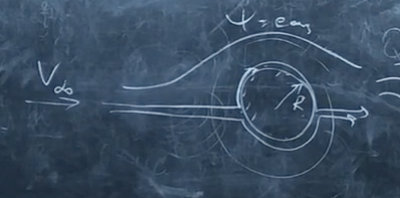
\includegraphics[width=0.2\textwidth]{14/pic_8.png}
	\caption{\label{ris:image14.8}}
\end{wrapfigure}

Рассмотрим $w=v_{\infty}(z + \frac{R^2}{z})$. Оно переводит окружность круга радиуса $R$ на некоторый отрезок . $w' = v_{\infty} ( 1 -  \frac{R^2}{z^2})$ , $w' \rightarrow v_{\infty} $ на бесконечности. Линии тока ведут себя как на рисунке 8. 

Также можем добавить к w функцию и рассмотреть следующий потенциал (круговые линии на рисунке 8 ) . Итого $w = v_{\infty}(z + \frac{R^2}{z}) + \frac{\Gamma}{2 \pi i} \ln z$. 

\begin{wrapfigure}{l}{0.15\textwidth}
	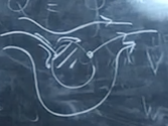
\includegraphics[width=0.15\textwidth]{14/pic_9.png}
	\caption{\label{ris:image14.9}}
\end{wrapfigure}
$$ $$

Вообще говоря $\Gamma$ произвольное, но надо выбрать единственное. По постулату Жуковского-Чаплыгина $\Gamma$ выбирается так чтобы в "острой", особенной точке скорость была равна нулю, то есть переходила в критическую точку. Таким образом можно выбрать единственное $\Gamma$. С гамма - циркуляцией получится картинка 9 с критической точкой (типа седло).

\newpage
\ \\

Рассмотрим произвольную функцию $w(z)$ и разложим в ряд Лорана $w' = ... + \frac{c_{-2}}{z^2} + \frac{c_{-1}}{z} + c_0 + c_1 z + c_2 z^2 + ... $. При устремлении z к бексонечности $w'$ должно получиться равным сопряженной скорости, таким образом $c_1 = c_2 = 0$, а $c_0 = \bar{v}_{\infty}$

Если взять циркуляцию от $w'$ , то получим $\Gamma = c_1 2 \pi i $ (по формуле) . $c_{-1} = \frac{\Gamma}{2 \pi i}$

\begin{wrapfigure}{r}{0.15\textwidth}
	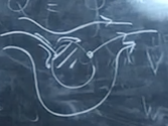
\includegraphics[width=0.15\textwidth]{14/pic_9.png}
	\caption{\label{ris:image14.10}}
\end{wrapfigure}
$$ $$

Чему равна сила , с действующая на данное тело ? 

Обозначим ее $R = X + i Y = - 	\oint \limits_{C} p \overrightarrow{n} d \overrightarrow{e} = - \oint \limits_{C} p e^(i\frac{pi}{2} + i\theta) d | \overrightarrow{e} |$ . Причем $p \in \mathbb{R}$

Что такое $dz$ ? $dz = e^{i \theta} d | \overrightarrow{e} |$, $w'$  в свою очередь, $w' = u -i \varv$ -  комплесносопряженная скорость 

Также вспомним интеграл Бернулли
$$ \begin{cases}
	p + p \frac{|v|^2}{2} = const \\
	v = u + i \varv
\end{cases},$$

Интеграл по кругу от константы по контуру равен нулю 

$- \oint \limits_{C} p e^(i\frac{pi}{2} + i\theta) d | \overrightarrow{e} | = -i \oint  \limits_{C} p dz = \frac{p i}{2} \oint  \limits_{C} |v|^2 dz =  \frac{p i}{2} \oint  \limits_{C} w' \bar{w}' d z$

Далее подробнее рассмотрим $w'$ , $\bar{w}' = v, \ \bar{d z} = e^{-i \theta} |d \overrightarrow{e} |$

$\bar{w}' \bar{dz} = |v| e^{i \theta} |d \overrightarrow{e} | e^{-i \theta} = w' dz$

$w' = ... + \frac{c_2}{z^2} + \frac{c_1}{z} + c_0 \ \rightarrow \ w'^2 = ... + \frac{2 c_1 c_0}{z} + ...$. Нас интересуют только вычеты , смотрим где $\frac{1}{z}$ 

В итоге получаем : 

$\bar{R} =  \frac{p}{2 i} \oint \limits_{C} \bar{w}'  w'  \bar{d z} =  \frac{p}{2 i} \oint \limits_{C} w'^2 dz =   \frac{p}{2 i} 2 c_{-1} c_0 2 \pi i = \rho c_{-1} c_0 2 \pi$

$ c_0 = \bar{v}_{\infty}$

$c_{-1} = \frac{\Gamma}{2 \pi i} $

Значит , $\bar{R} = - \rho \frac{\Gamma}{i} v_{\infty} $ (- на лекциях где-то потеряли, ну а я писал конспект по лекциям)

В итоге , Формула Жуковского 

$$
R = -i \rho v_{\infty} \Gamma
$$

Если скорость направлена в точности по оси x (то есть действительная часть равна 0) , то 

$X = 0$ - парадокс Даламбера , сила , действуюшая по направлению набегающей скорости равна нулю

$Y = -\rho v_{\infty} \Gamma $ - подъемная сила. Сила , напраленная перпендикулярно набегающей скорости , пропорциональна скорости и завихренности . Чем больше завихренности крыла, тем больше сила . 
\input {15/15_ticket.tex}
\newpage
\section{Билет 16. Вязкая жидкость. Закон Навье-Стокса. Уравнения Навье-Стокса. Полная система уравнения, описывающая движение вязкой несжимаемой жидкости. Течение Пуазейля. Течение Куэтта. Закон Фурье. Полная система уравнений, описывающая движение вязкого теплопроводного совершенного газа.}

\begin{center}
	\textit{\underline{Вязкая жидкость}}
\end{center}

\begin{defn}
	Жидкость или газ называются \textbf{вязкими}, если в них при движении, возможно касательные напряжения. В таком случае компоненты тензора напряжений в вязкой жидкости представляются в виде: $$p^{ij}=-pg^{ij} + \tau^{ij},  \tau^{ij} = \tau^{ij}(e_{kl}, T) ,$$
	где $p$-давление, $e_kl$ - компоненты тензора скоростей деформаций, $T$-температура. 
\end{defn}

\begin{defn}
	\textbf{Компонентами тензора вязких напряжений} называются $\tau^{ij}$.
\end{defn}

Заметим, что если жидкость покоится, то $\tau^{ij} = 0$.

\begin{defn}
	Жидкость или газ называются \textbf{линейно-вязкими (или ньютоновскими)}, если $\tau^{ij}$ являются линейными функциями компонент тензора скоростей деформации ($e_{kl}$), т.е.: $$\tau^{ij} = A^{ijkl}e_{kl}, $$ где $A^{ijkl}$-коэффиценты вязкости.
\end{defn}


Ньютон в своем опыте с двумя пластинами выявил такую характеристику жидкости или газа, как вязкость.  Это свойство жидкости проявляется лишь при ее движении. Допустим, что некоторое количество жидкости заключено между двумя плоскими неограниченными параллельными пластинами; расстояние между ними – $d$; скорость движения верхней пластины относительно нижней – $v_0$.

Опыт показывает, что слой жидкости, непосредственно прилегающий к стенке, прилипает к ней. Отсюда следует, что скорость движения жидкости, прилегающей к нижней стенке, равна нулю, а к верхней – $v_0$. Промежуточные слои движутся со скоростью, постепенно возрастающей от $0$ до $v_0$.

Чтобы перемещать одну пластину относительно другой, необходимо приложить к движущейся пластине некоторую силу $F$, равную силе сопротивления жидкости в результате внутреннего трения. Ньютон установил, что эта сила пропорциональна скорости $v_0$, поверхности соприкосновения $S$ и обратно пропорциональна расстоянию между пластинами $d$ т.е.:
$$F = \mu\frac{S v_0}{d}$$

\begin{figure}[H]
	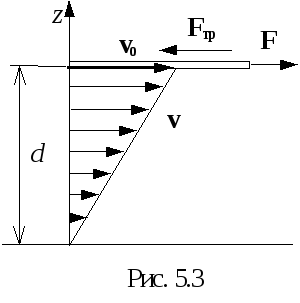
\includegraphics[width=0.4\textwidth]{16/newton_experiment.png}
\end{figure}


\begin{center}
	\textit{\underline{Закон Навье-Стокса}}
\end{center}


\begin{defn}
	\textbf{Изотропность} - совпадение свойства по всем направлениям. 
\end{defn}

\begin{theorem}[Э-132]Закон Навье-Стокса
	Для изотропных, линейно-вязких жидкостей верно следующее утверждение:
	$$\tau^{ij} = \lambda I_1(e)g^{ij}+2\mu e^{ij},$$ где $\lambda$, $\mu$ - коэффиценты вязкости, $I_1(e) = e_{ij}g^{ij}$ - первый инвариант тензора скоростей деформаций.
\end{theorem}


\begin{center}
	\textit{\underline{Уравнения Навье-Стокса}}
\end{center}

Уравнения движения линейно-вязких жикостей или газов называется уравнением Навье-Стокса. Они получаются из универсальных газовых уравнений: $$\rho\frac{dv^i}{dt} = \rho F^i + \nabla_{i}p^{ij}$$ подстановкой выражений для $p^{ij}$ и $\tau^{ij}$ и выведением уравнений покомпонентно.

Итоговое уравнение Навью-Стокса:

$$\frac{dv}{dt} = \hat{F} - \frac{1}{\rho}grad p + \frac{\lambda + \mu}{\rho}grad(div \hat{v}) + \frac{\mu}{\rho}\Delta \hat{v}$$


\begin{center}
	\textit{\underline{Полная система уравнения, описывающая движение вязкой несжимаемой жидкости}}
\end{center}


Полна система механических уравнений для несжимаемой линейно-вязкой жидкости с постоянными коэффицентами вязкости состоит из уравнения неразрывности, условия несжимаемости и уравнения Навье-Стокса:

\begin{equation} \label{eq:task}
	\begin{cases}
		\begin{array}{l}
			div \, \hat{v} = 0\\
			\frac{d\rho}{dt} = \frac{\partial \rho}{\partial t} + v^k\frac{\partial \rho}{\partial x^k} = 0\\
			\frac{dv}{dt} = \hat{F} - \frac{1}{\rho}grad\, p + \frac{\mu}{\rho}\Delta \hat{v}
		\end{array}
	\end{cases}
\end{equation}

\begin{center}
	\textit{\underline{Течение Пуазейля}}
\end{center}

\begin{defn}
	\textbf{Течение Пуазейля} - ламинарное течение жидкости через каналы в виде прямого кругового цилиндра или слоя между параллельными плоскостями. Течение Пуазёйля — одно из самых простых точных решений уравнений Навье — Стокса. Описывается законом Пуазёйля (также называемым законом Гагена — Пуазёйля или Хагена — Пуазёйля).
\end{defn}

\begin{figure}[H]
	\centering
	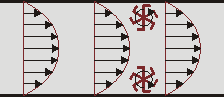
\includegraphics[width=0.4\textwidth]{16/poiseuille_profile.png}
\end{figure}

Течение Пуазёйля характеризуется параболическим распределением скорости по радиусу трубки. В каждом поперечном сечении трубки средняя скорость вдвое меньше максимальной скорости в этом сечении.


\begin{center}
	\textit{\underline{Течение Куэтта}}
\end{center}

\begin{defn}
	\textbf{Течение Куэтта} - ламинарное течение вязкой жидкости между двумя параллельными стенками (не обязательно прямолинейными), одна из которых двигается относительно другой. Течение происходит под действием сил вязкого трения, действующих на жидкость, и сдвигового напряжения параллельного стенкам.
\end{defn}



\input {17/17_ticket.tex}
\input {18/18_ticket.tex}
\newpage
\section{Билет 19. Постановка задач теории упругости в перемещениях и напряжениях. Граничные условия. Принцип Сен-Венана.}

\subsection{В перемещениях}
Если на границе тела заданы перемещения, удобно в качестве основных уравнений брать уравнения теории упругости в перемещениях, которые называются уравнениями Навье-Ламе. Они получаются из общих уравнений количества движения с использованием закона Гука и формул, выражающих компоненты тензора деформации через перемещения. Уравнения Навье-Ламе выглядят следующим образом:
$$
\rho_0\frac{\partial^2 w^i}{\partial t^2} = \rho_0 F^i + (\lambda + \mu)g^{ij}\nabla_j \mathrm{div} \vec{w} + \mu \Delta w^i
$$

Если на поверхности тела заданы перемещения, то из уравнений Навье-Ламе определяется вектор $w$ и этим решается задача о равновесии упругого тела в перемещениях. Напряжения при этом могут быть найдены согласно закону Гука. 

\subsection{В напряжениях}

При решении задачи в напряжениях, используются уравнения равновесия в напряжениях  $$\rho_0 F^i + \nabla_j p^{ij} = 0$$, эти три уравнения содержат шесть неизвестных компонент тензора напряжений и составляют незамкнутую систему. В некоторых случаях, например из симметрии задачи, можно заранее понять, что в эти уравнения входят только три неизвестные компоненты напряжений и если на границе известны $p_n$, то можно найти напряжения используя только эти три уравнения.

В общем случае, с помощью закона Гука из уравнений совместности деформаций можно получить дополнительные уравнения, которым должны удовлетворять компоненты тензора напряжений. Эти уравнения называются уравнениями Бельтрами-Мичелла, и выглядят следующим образом:
$$
\Delta p_{ij} + \frac{1}{1+\sigma} \frac{\partial^2 \wp}{\partial x^i \partial x^j}
$$
Причем в декартовых координатах $\wp = p_{11} + p_{22} + p_{33}$.

\newpage
\subsection{Граничные условия}

Граничные условия в задачах теории упругости бывают трёх оснонвх типов:
\begin{enumerate}
\item Граничные условия первого рода: задан вектор $\vec{w}$ на всей поверхности тела $\Sigma$
\begin{center}
$\vec{w}\mid_{\Sigma} = \vec{f}(x^i,t)$, где $\vec{f}$ - заданная функция
\end{center}

\item Граничные условия второго рода: на поверхности тела $\Sigma$ задан вектор напряжений $\vec{P_n}$ как функция времени и координат точек поверхности
\begin{center}
$\vec{P_n}\mid_{\Sigma} = \vec{\varphi}(x^i,t)$, где $\vec{\varphi}$ - заданная функция
\end{center}

\item Граничные условия третьего рода: на одной части поверхности тела  $\Sigma_w$ задан вектор $\vec{w}$, а на другой части  $\Sigma_p$ - $\vec{P_n}$
\begin{center}
$\vec{w}\mid_{\Sigma_w} = \vec{f}$ \ \ \ \ \  $\vec{P_n}\mid_{\Sigma_p} = \vec{\varphi}$
\end{center}
\end{enumerate}

\subsection{Принцип Сен-Венана}

\begin{wrapfigure}{R}{0.4\textwidth}
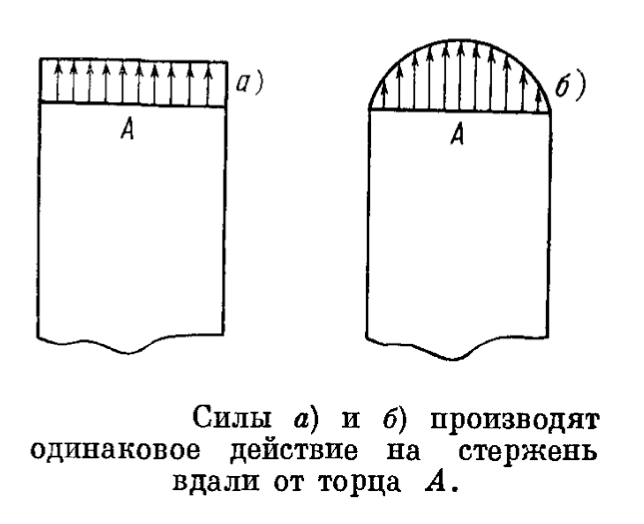
\includegraphics[width=0.4\textwidth]{19/sen_venan.png}
\end{wrapfigure}

Если в некоторой области внутри или на поверхности тела, малой по сравнению с основными размерами тела, на него действует система массовых или поверхностных сил и тело находится в равновесии, то в областях, удаленных от места приложения этих сил, деформированное и напряженное состояния определяются в основном только главным вектором и главным моментом этих сил и приближенно не зависят от детального характера распределения сил. Влияние деталей распределения сил практически сказывается только в непосредственной окрестности области их приложения.

\input {20/20_ticket.tex}
\input {21/21_ticket.tex}

\newpage
\begin{thebibliography}{100}
	
\end{thebibliography}

\end{document}
